% 编辑器使用说明

\subsection{简介}
\begin{itemize}
\item 在线编辑器网址为 \href{http://wuli.wiki/editor}{wuli.wiki/editor}, 也可从网站首页的链接进入
\item 编辑器处于测试阶段, 请自行使用下载按钮备份
\item 该编辑器可直接将 LaTeX 代码转换为 html 网页而不是 pdf
\item 我们以后也会开发在线编译 pdf 并下载的功能
\item 该编辑器除公式外只支持有限的 LaTeX 命令(工具栏有一些常用的)
\item 我们在模板中加入了许多自定义命令, 但不会覆盖原有的 LaTeX 命令
\item 正文中支持的所有命令见 “词条示例\upref{Sample}”
\item 正文中请使用中文标点, 编辑器会自动把空心句号替换为全角实心句号
\end{itemize}

\subsection{公式}
\begin{itemize}
\item 公式环境支持大部分 LaTeX 命令, 严格来说是所有 \href{https://www.mathjax.org/}{MathJax} 支持的命令\footnote{MathJax 项目用于在网页上显示 LaTeX 公式}
\item 一个简单的公式编辑器见\href{https://www.codecogs.com/latex/eqneditor.php}{这里}
\item 一个简单的 TeX/LaTeX 入门教程见\href{https://chaoli.club/index.php/211}{超理论坛}
\item 支持部分\href{http://mirrors.ibiblio.org/CTAN/macros/latex/contrib/physics/physics.pdf}{Physics 宏包}中的命令
\item 行内公式只能用美元符号
\item 独立公式用 equation 环境, align 环境或者 gather 环境
\item 公式中所有常用的和自定义的命令见 “词条示例\upref{Sample}”
\end{itemize}

\subsection{百科的结构}

百科的所有词条是 LaTeX 的一个 document 环境, 每个部分是一个 \lstinline|\part|, 每章是一个 \lstinline|\chapter|, 词条是 \lstinline|\section|, 蓝色的小标题是 \lstinline|\subsubsection|, 黑色的小标题是 \lstinline|\subsubsection|. 编辑器打开的一个词条文件就是一个 section. 用 texlive 编译 pdf 的时候所有 section 都会通过 \lstinline|\input| 插入到主文件 PhysWiki.tex 中.

网页版的词条目录(\href{http://wuli.wiki/online/}{wuli.wiki/online/})由 PhysWiki.tex 生成, 所以发布词条后必须修改该文件并发布才能在目录中显示.

每个注册用户默认有编辑词条的权限, 但却不能直接发布词条, 而是需要由发布权限的用户审核后发布. 所有编辑中的词条页面都在 \href{http://wuli.wiki/changed/}{wuli.wiki/changed/} 目录下. 若要查看所有编辑中词条的目录, 可以用 \href{http://wuli.wiki/changed/changed.html}{wuli.wiki/changed/changed.html}(见\autoref{editor_fig1}).

\begin{figure}[ht]
\centering
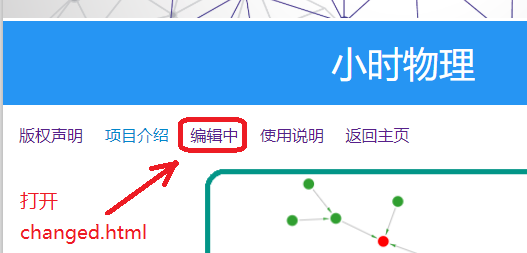
\includegraphics[width=9cm]{./figures/editor1.png}
\caption{从 \href{http://wuli.wiki/online}{wuli.wiki/online} 查看编辑中的词条} \label{editor_fig1}
\end{figure}

每个词条文件(后缀名为 tex)都有一个独一无二的文件名, 可以将通过将光标停留在编辑器中的 tab 上查看.

\begin{figure}[ht]
\centering
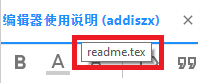
\includegraphics[width=4cm]{./figures/editor2.png}
\caption{查看词条文件名} \label{editor_fig2}
\end{figure}

每个词条(section) 的 label 与文件名相同, 转换后输出的 html 文件也由相同的文件名, 可以在浏览器的地址栏中看到(例如本文的 tex 文件是 editor.tex, label 是 editor, 转换成网页为 editor.html).

\subsection{编辑器说明}
\begin{itemize}
\item 将光标停留在任意按钮上都会出现提示说明按钮的名称. 要新建词条, 点击红色的加号按钮, 根据提示新建即可. 要打开已有词条, 点击最右边的打开, 搜索需要的词条即可

\item 按下保存按钮(快捷键 \lstinline|Ctrl + s|) 会自动保存并编译

\item 编辑器支持各种自动引用(被引用对象没有 label 时会自动插入 label), 工具栏上的内部引用按钮可以引用同一词条的公式, 图表, 例题等环境. 外部引用按钮可以引用其他词条的各种环境

\item 如果要在 html 预览和 LaTex 代码之间跳转, 可以通过搜索关键词实现. 例如在预览窗口复制一段文字, 在编辑窗口搜索就可以跳转到对应内容

\item 任何时候打出反斜杠会自动提示, 用 tab 键自动补全, 用上下键选择. 候选词未必是从最左边开始匹配, 例如打 \lstinline|\bf| 按 tab 就会得到 \lstinline|\textbf|

\item 如果自动补全带括号, 例如 \lstinline|\frac{}{}|, 补全后光标会自动进入第一个大括号, 再次按 tab 光标会跳到第二个括号, 再按 tab 光标会跳到第二个大括号外.

\item 打 \lstinline|\beg| 按 tab 会自动出现 \lstinline|\begin{}...\end{}|, 在 \lstinline|begin| 中输入环境名时, \lstinline|end| 中的环境名也会同步. 输完以后按 tab, 光标会跳到环境内
\end{itemize}

\subsubsection{快捷键}

\begin{table}[ht]
\centering
\caption{编辑器快捷键}\label{editor_tab1}
\begin{tabular}{|c|c|c|c|}
\hline
保存词条 & \lstinline|Ctrl + S| & 打开词条 & \lstinline|Ctrl + O| \\
\hline
新建词条 & \lstinline|Ctrl + Alt + N| & 关闭词条 & \lstinline|Ctrl + Alt + W| \\
\hline
显示编辑器选项 & \lstinline|Ctrl + Q| & 跳转到某行 & \lstinline|Ctrl + L| \\
\hline
查找文本 & \lstinline|Ctrl + F| & 替换文本 & \lstinline|Ctrl + H| \\
\hline
向左缩进 & \lstinline|Ctrl + [| & 向右缩进 & \lstinline|Ctrl + ]| \\
\hline
增大字号 & \lstinline|Shift + Alt + (+)| & 减小字号 & \lstinline|Shift + Alt + (-)| \\
\hline
关闭不保存 & \lstinline|Shift + 点关闭| &  &  \\
\hline
\end{tabular}
\end{table}
